\documentclass[handout]{beamer} % [handout] para imprimir eliminando transiciones

%\usefonttheme[onlymath]{serif}
%\usepackage{fontspec}
%\defaultfontfeatures{Mapping=tex-text}
%\setsansfont[Ligatures={Common}]{Futura}
%\setmonofont[Scale=0.8]{Monaco} 

\usepackage{beamerthemesplit}
\usepackage[utf8]{inputenc}
\usepackage[spanish]{babel}
\mode<presentation>
\usetheme{default}
\usecolortheme{dolphin}
\usepackage{alltt}                                    % \begin{alltt}
\usepackage{amssymb}                                  % mathematical symbols
\usepackage{comment}
\usepackage{url}
\usepackage{tabto}                                    % \tabto
\usepackage{tikz}
\usetikzlibrary{automata}
\usetikzlibrary{positioning}
\usetikzlibrary{calc}

\usepackage{verbatim}                                 % comentarios

\title{Lenguajes de Programación}                     %[titulo corto]
\author{Fabián Riquelme Csori}                        %[nombre corto]
\date{2017}                                           %[fecha corta]
\institute{Universidad de Valparaíso}                 %[instituto corto]

\newcommand{\HRule}{\rule{\linewidth}{0.2mm}\\[1ex]}
\newcommand{\blue}[1]{\textcolor{blue}{#1}}
\newcommand{\red}[1]{\textcolor{red}{#1}}
\newcommand{\redb}[1]{{\color{red!70!black}{#1}}}
\newcommand{\green}[1]{{\color{green!70!black}{#1}}}
\newcommand{\gray}[1]{{\color{gray!50!white}{#1}}}
\newcommand{\yell}[1]{{\color{yellow!70!black}{#1}}}
\newcommand{\lQ}{\mbox{``}}
\newcommand{\rQ}{\mbox{''}}
% \alert{texto destacado en rojo}
% \color{green} Color en verde
% \structure{texto en lila}


\begin{document}

%\begin{frame}%[plain]
%  \titlepage
%\end{frame}
%
% [opciones]:
% plain: oculta barra de navegacion, deja + espacio para contenido
% fragile: usar comandos como verbatim
% b,c,t: alineacion vertical
% label=nombre_etiqueta
% allowframebreaks: divide contenido en varios frames si es demasiado largo
% shrink: para escribir mucho texto en una transparencia, reduciendo tamano de fuente

%%%%%%%%%% PORTADA %%%%%%%%%%
\begin{frame}[plain]
  \begin{figure}[h]
    \begin{minipage}{0.3\textwidth}
    
\includegraphics[width=.9\textwidth]{./image/logo-UV.png}
    \end{minipage}
    \begin{minipage}{0.65\textwidth}
     $~$\\[3.6ex]
     \footnotesize{Escuela de Ingeniería Civil Informática}\\
     \footnotesize{Facultad de Ingeniería}
    \end{minipage}
  \end{figure}
  \begin{center}
    \vspace{1ex}
    \HRule
    \Large{Lenguajes de Programación}\\{\small Capítulo VII: Concurrencia}\\[-1ex]
    \HRule\vspace{1ex}
    \large{Fabián Riquelme Csori}\\[.5ex]\footnotesize{fabian.riquelme@uv.cl}\\[6ex] {\tiny 2017-II}\\[6ex]
  \end{center}
\end{frame}

%%%%%%%%%% INDEX %%%%%%%%%%
\begin{frame}
 \frametitle{Index}
 \scriptsize 			% reducir tamano de letra
 \tableofcontents		%[pausesections]
\end{frame}

%%%%%%%%%%% ACTUAL INDEX %%%%%%%%%%
%\AtBeginSection[] %generar indice automaticamente
%{
%\begin{frame}<beamer>%[plain]
% \frametitle{Index}
% \framesubtitle{subtitulo}
% \scriptsize
% \tableofcontents[currentsection, currentsubsection]
%\end{frame}
%}

%==============================
\section{Concurrencia}

%------------------------------
\subsection{Programación concurrente}

\begin{frame}{Breve historia}
  \begin{itemize}
    \item La programación concurrente está íntimamente asociada a los sistemas operativos.
    \item Se comenzó a desarrollar con Dijkstra (1965), inspirada en ferrocarriles, telégrafos y semáforos.
    \item Inicialmente se programaba a bajo nivel (ensamblador).
  \end{itemize}
\end{frame}

\begin{frame}{Para evitar confusiones...}

  Diferenciemos entre \blue{programación concurrente}, \blue{programación paralela} y \blue{sistema distribuido}:
  \begin{itemize}
    \item<2-> La \blue{programación concurrente} consiste en la ejecución de \redb{múltiples procesos} durante un mismo período de tiempo.
    \begin{itemize}
        \item Ej: clientes pidiendo acceso simultáneo a un servidor.
    \end{itemize}
    \item<3-> La \blue{programación paralela} es un caso particular de concurrencia, cuando procesos se ejecutan al mismo tiempo.
    \begin{itemize}
        \item Ej: uso de multi-procesadores.
        \item Ej: comunicación en sistemas distribuidos.
    \end{itemize}
    \item<4-> Observemos estos dos casos:
    \begin{itemize}
        \item $x=x+1;$\\$y=x+1;$
        \item int $x=1$, $y=2$, $z=3$;
    \end{itemize}
  \end{itemize}
\end{frame}

\begin{frame}{Para evitar confusiones...}
  
  Distingamos ahora entre \blue{programa} y \blue{proceso}:
  \begin{itemize}
    \item<2-> Un \blue{programa} es un conjunto de sentencias/instrucciones que se ejecutan secuencialmente.
    \begin{itemize}
        \item Es un concepto \redb{estático}, semejante a noción de {\em clase} en POO.
    \end{itemize}
    \item<3-> Un \blue{proceso} es un programa o subprograma en ejecución.
    \begin{itemize}
        \item Un programa se puede subdividir en procesos.
        \item Son líneas de código que se ejecutan de manera \redb{dinámica}.
        \item Es un concepto semejante a noción de {\em objeto} en POO.
    \end{itemize}
  \end{itemize}
  \uncover<4->{
  \begin{center}
    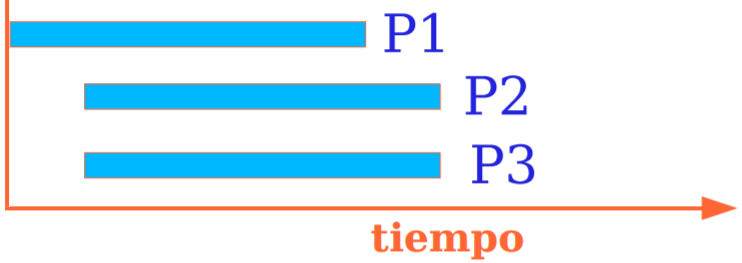
\includegraphics[width=.5\textwidth]{./image/cap7/concurrency.png}
  \end{center}}
  \begin{itemize}
    \item<5-> Los procesos compiten o colaboran entre sí por los recursos del sistema, mediante tareas de \blue{sincronización} y \blue{colaboración}.
  \end{itemize}
\end{frame}

\begin{frame}{Ventajas y aplicaciones}
  \begin{itemize}
    \item<2-> Mejoras en el rendimiento de programas.
    \item<2-> Alta capacidad de respuesta I/O.
    \item<2-> Adaptación natural a varios contextos:
    \begin{itemize}
        \item Sistemas de control (Ej: sistemas de tiempo real)
        \item Servidores web
        \item Aplicaciones GUI (Ej: navegadores web)
        \item Simuladores
        \item Sistemas de gestión de bases de datos, etc.
    \end{itemize}
  \end{itemize}
\end{frame}

\begin{frame}{¿Qué procesos pueden ser concurrentes?}
  \begin{itemize}
      \item<1-> Dado un proceso \blue{$P$}, decimos que \blue{$I$} es su conjunto de variables de entrada y \blue{$O$} su conjunto de variables de salida.
      \begin{itemize}
          \item Ej: si $P_1$ es \redb{$a=x+y$;} entonces \uncover<2>{$I_1=\redb{\{x,y\}}$ y $O_1=\redb{\{a\}}$.}
      \end{itemize}
  \end{itemize}
  \uncover<3->{
  \begin{block}{Condiciones de Bernstein}
    \begin{itemize}
    \item<3-> Dos procesos $P_i$ y $P_j$ son independientes, y por tanto pueden ejecutarse concurrentemente, si:
      \begin{itemize}
        \item $\,\, I_i\, \cap O_j=\emptyset$
        \item $\,\, I_j\, \cap O_i=\emptyset$
        \item $O_i\cap O_j=\emptyset$
      \end{itemize}
    \end{itemize}
  \end{block}}
  \uncover<3->{\begin{flushright}
  {\scriptsize Bernstein, AJ (1966). Analysis of Programs for Parallel Processing.\\{\em IEEE Transactions on Electronic Computers}, EC-15(5): 757-763.}\end{flushright}}
\end{frame}

\begin{frame}{¿Qué procesos pueden ser concurrentes?}
  \begin{block}{Ejercicio}
    Utilizando las condiciones de Bernstein, determine qué procesos de los siguientes pueden ejecutarse concurrentemente.
    \begin{itemize}
        \item $P_1$: $a=x+y$;
        \item $P_2$: $b=z-1$;
        \item $P_3$: $c=a-b$;
        \item $P_4$: $w=c+1$;
    \end{itemize}
  \end{block}
\end{frame}

\begin{frame}{Características de los sistemas concurrentes}
    \begin{itemize}
        \item<1-> \blue{Orden de ejecución}: orden solo parcialmente secuencial,\\lo que genera...
        \item<1-> \blue{Indeterminismo}: distintas ejecuciones producen distintos comportamientos o resultados.
        \begin{itemize}
            \item<2-> Pregunta: ¿en qué se diferencia el indeterminismo del \blue{no-determinismo}?
        \end{itemize}
    \end{itemize}
\end{frame}

\begin{frame}{Condiciones de carrera}
    \begin{itemize}
        \item<1-> Bugs generados por \blue{condición de carrera} (\blue{\em race condition}).
        \begin{itemize}
            \item<2-> Ej: Eliminar concurrentemente dos nodos de una lista enlazada.
            \medskip
            
            \begin{center}
              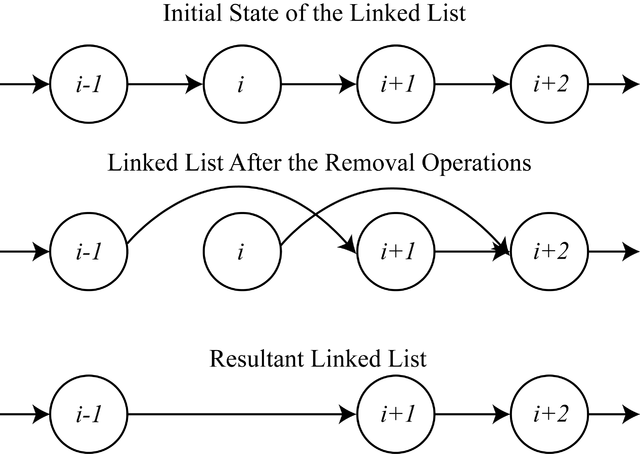
\includegraphics[width=.6\textwidth]{./image/cap7/mutual-exclusion.png}
            \end{center}
            \smallskip
        \end{itemize}
        \item<3-> Solución: \blue{Exclusión mutua} (\blue{\em mutual exclusion}) $\to$ Buscar...
    \end{itemize}
\end{frame}

\begin{frame}{Ciclo de vida de un proceso}
    \begin{center}
        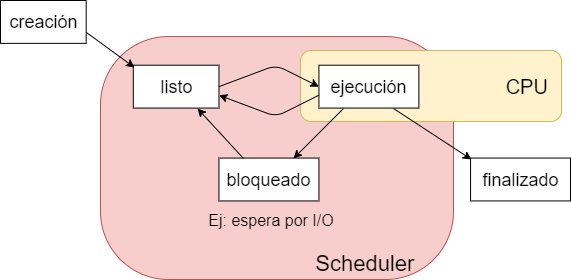
\includegraphics[width=.9\textwidth]{./image/cap7/ciclo-vida.png}
    \end{center}
\end{frame}

\begin{frame}{Disposición de memoria de un proceso}
    \begin{center}
        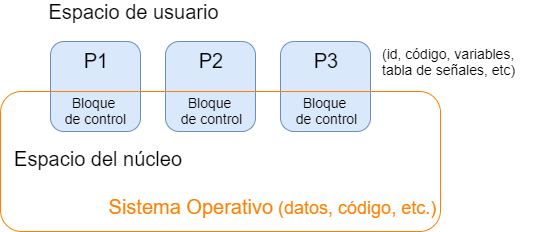
\includegraphics[width=.8\textwidth]{./image/cap7/espacios-procesos.png}
    \end{center}
    \begin{itemize}
        \item<2-> Cada proceso tiene sus propias características: id, código, variables, contadores, pila, etc.
        \item<3-> Cada proceso es \blue{monohilo} o \blue{\em mono thread}.
        \item<4-> La gestión y cambio de contexto de cada proceso es muy costoso. Se deben actualizar registros de uso de memoria y controlar estados finales de los procesos.
        \begin{itemize}
            \item<5-> Solución: utilizar \redb{procesos de procesos} (\blue{hebras}/\blue{hilos}/\blue{\em threads}).
        \end{itemize}
    \end{itemize}
\end{frame}

\begin{frame}{Ejercicio}
    \begin{itemize}
        \item Busque algún código que implemente un \blue{semáforo}\\(TDA usado para controlar el acceso concurrente de varios procesos a un mismo recurso).
        \item Observe el código y vea cómo aplica la {\em exclusión mutua}.
        \item ¿Qué es un \blue{deadlock}? ¿Es dicho código capaz de evitarlos?
    \end{itemize}
\end{frame}

%------------------------------
\subsection{Hebras}

\begin{frame}{Hebras/Hilos/Threads}
    \begin{itemize}
        \item Una \blue{hebra} es una secuencia de control dentro de un proceso que ejecuta sus instrucciones de forma independiente.
    \end{itemize}
    \begin{center}
        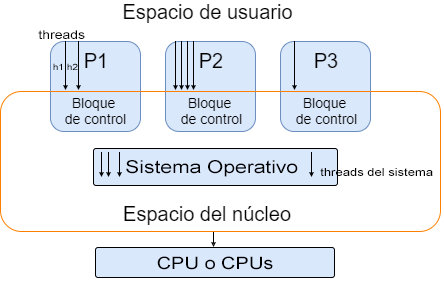
\includegraphics[width=.8\textwidth]{./image/cap7/espacios-hebras.png}
    \end{center}
\end{frame}

\begin{frame}{Niveles de hebras}
    \begin{itemize}
        \item Las hebras pueden estar a \blue{nivel de usuario} (Ej: Java)\\o a \blue{nivel del sistema operativo} (Ej: hebras de sistema).
        \item Los segundos dan soporte a los primeros mediante una API.
        \item Cada SO implementa las hebras de sistema de modo distinto:
        \begin{itemize}
            \item \blue{Windows API} (basada en \blue{win32})
            \item \blue{OS/2 API}
            \item \blue{POSIX} (\blue{pthreads}).
        \end{itemize}
        \item Se pueden implementar a nivel usuario
        \begin{itemize}
            \item Ej: en Java, con clase Threads del paquete \blue{java.lang.Thread} o bien objeto ExecutorService de paquete \blue{java.util.concurrent)}.
        \end{itemize} o a nivel de núcleo (llamadas a sistema).
    \end{itemize}
\end{frame}

\begin{frame}{Ejercicio: Hebras en Java (parte 1)}
    \begin{itemize}
        \item Se desea simular un proceso de ingeniería de software mediante programación concurrente. {\scriptsize Info útil:\\ \blue{\url{http://dalila.sip.ucm.es/~manuel/JSW1/Slides/Concurrencia.pdf}}}
        \item El equipo de trabajo está conformado por: 1 analista,\\1 diseñador, 2 programadores y 1 encargado de testing.
        \item Cada uno posee un nivel de avance, que va de 0-100\%.
        \item Simule los niveles de avance del proyecto, si todos trabajan concurrentemente partiendo de 0\% hasta alcanzar su 100\%.
    \end{itemize}
\end{frame}

\begin{frame}{Ejercicio: Hebras en Java (parte 2)}
    \begin{itemize}
        \item Con lo anterior, obviamente el producto final será un desastre...
        \item Repita el experimento anterior, pero esta vez los programadores solo pueden acabar su tarea una vez que el analista y el diseñador hayan alcanzado su 100\% de avance.
    \end{itemize}
    \begin{flushright}
        \red{[bonus +1]}
    \end{flushright}
\end{frame}

\begin{frame}{Ejercicio: Hebras en Java (parte 3)}
    \begin{itemize}
        \item Repita el experimento anterior, pero esta vez centrémonos en el porcentaje de avance del proyecto total.
        \item Los miembros del equipo se dividen el proyecto de esta manera:
        analista (20\%), diseñador (20\%), programadores (25\% c/u) y encargado de testing (10\%).
        \item Simule esta vez el avance del proyecto mediante un contador de porcentaje común a todas las hebras. El proyecto se considera terminado si se alcanza entre todos los miembros del equipo el 100\% de avance, y ninguno trabaja más de su porcentaje de trabajo asignado.
    \end{itemize}
    \begin{flushright}
        \red{[bonus +1]}
    \end{flushright}
\end{frame}

%------------------------------

\begin{frame}
 \begin{block}{Bibliografía}
  \begin{itemize}
    \item Pratt, Terrence W. (1998). \textit{Lenguajes de programación: diseño e implementación}, Pearson Education.
    \item Sethi, Ravi (1992). \textit{Lenguajes de programación: conceptos y constructores}, Addison-Wesley Iberoamericana.
    \item Scott, Michael (2009). \textit{Programming Language Pragmatics}, Morgan Kaufman, 3ra ed.
  \end{itemize}
 \end{block}
 \begin{block}{Recursos}
  \begin{itemize}
    \item Wikipedia y Wikimedia Commons.
    \item Apuntes de Miguel Ángel Rodríguez Florido, Departamento de Ingeniería Telemática, U. Las Palmas de Gran Canaria.
  \end{itemize}
 \end{block}
\end{frame}

\end{document}
